\documentclass{standalone}
\usepackage{tikz}
\usetikzlibrary{patterns, positioning}


\begin{document}
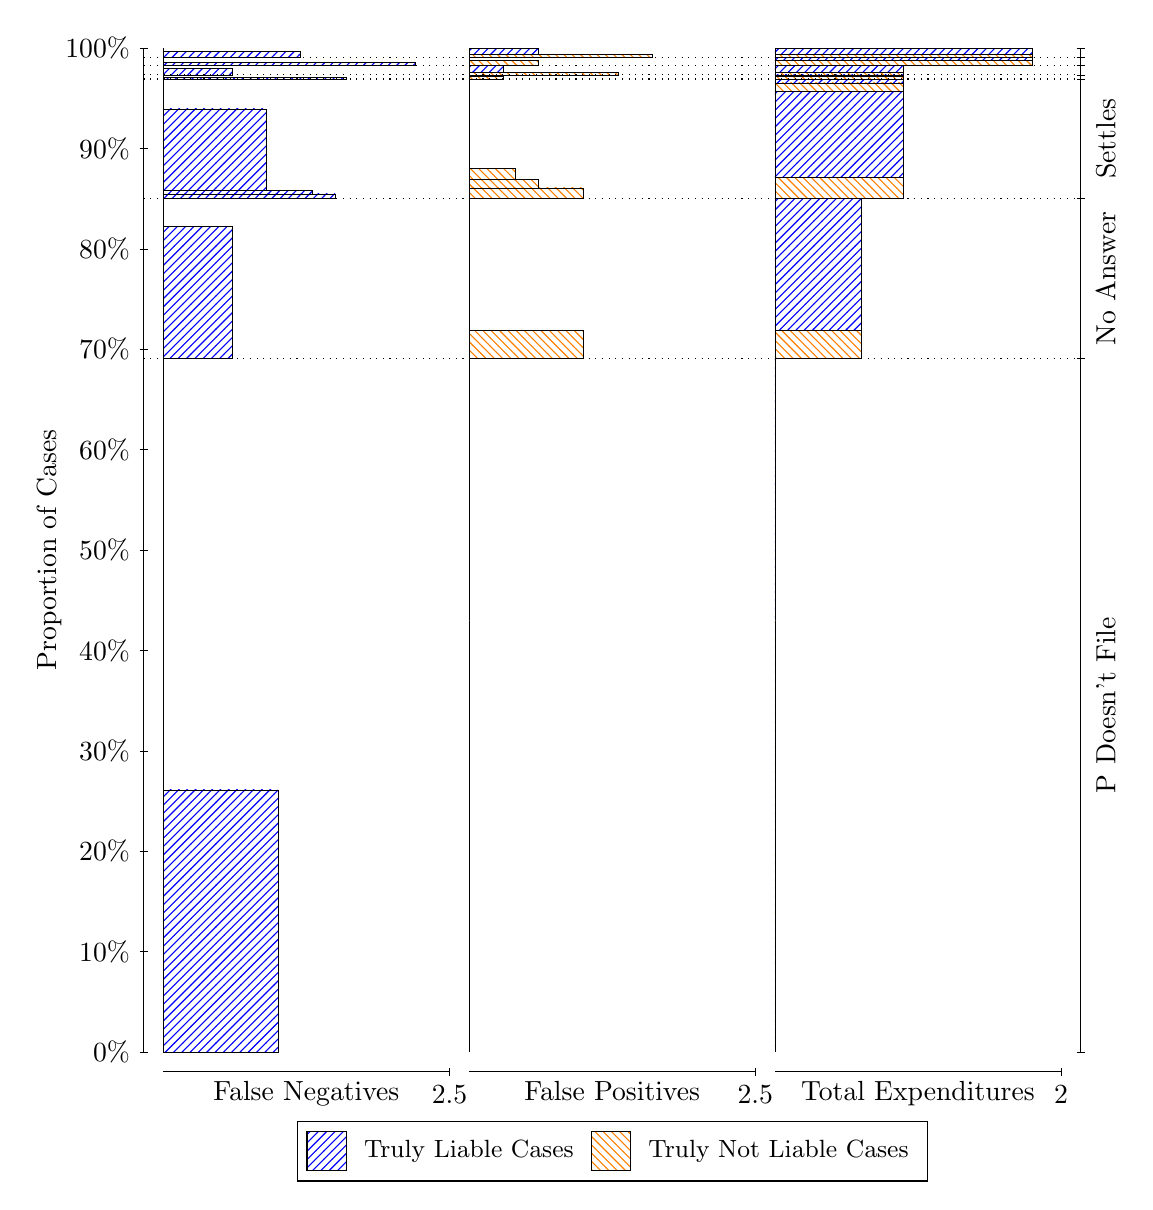
\begin{tikzpicture}
\draw[black, very thin] (1.5,1.75) -- (1.5,14.5);
\node[rotate=90, text=black, anchor=center] at (0.3, 8.125) {Proportion of Cases};
\draw[black, very thin] (1.45,1.75) -- (1.55,1.75);
\node[text=black, anchor=east] at (1.45, 1.75) {0\%};
\draw[black, very thin] (1.45,3.025) -- (1.55,3.025);
\node[text=black, anchor=east] at (1.45, 3.025) {10\%};
\draw[black, very thin] (1.45,4.3) -- (1.55,4.3);
\node[text=black, anchor=east] at (1.45, 4.3) {20\%};
\draw[black, very thin] (1.45,5.575) -- (1.55,5.575);
\node[text=black, anchor=east] at (1.45, 5.575) {30\%};
\draw[black, very thin] (1.45,6.85) -- (1.55,6.85);
\node[text=black, anchor=east] at (1.45, 6.85) {40\%};
\draw[black, very thin] (1.45,8.125) -- (1.55,8.125);
\node[text=black, anchor=east] at (1.45, 8.125) {50\%};
\draw[black, very thin] (1.45,9.4) -- (1.55,9.4);
\node[text=black, anchor=east] at (1.45, 9.4) {60\%};
\draw[black, very thin] (1.45,10.675) -- (1.55,10.675);
\node[text=black, anchor=east] at (1.45, 10.675) {70\%};
\draw[black, very thin] (1.45,11.95) -- (1.55,11.95);
\node[text=black, anchor=east] at (1.45, 11.95) {80\%};
\draw[black, very thin] (1.45,13.225) -- (1.55,13.225);
\node[text=black, anchor=east] at (1.45, 13.225) {90\%};
\draw[black, very thin] (1.45,14.5) -- (1.55,14.5);
\node[text=black, anchor=east] at (1.45, 14.5) {100\%};

\draw[black, very thin] (13.4,1.75) -- (13.4,14.5);
\draw[black, very thin] (13.35,1.75) -- (13.45,1.75);
\node[anchor=west] at (13.35, 1.75) {};
\draw[black, very thin] (13.35,10.56) -- (13.45,10.56);
\node[anchor=west] at (13.35, 10.56) {};
\draw[black, very thin] (13.35,12.587) -- (13.45,12.587);
\node[anchor=west] at (13.35, 12.587) {};
\draw[black, very thin] (13.35,14.106) -- (13.45,14.106);
\node[anchor=west] at (13.35, 14.106) {};
\draw[black, very thin] (13.35,14.16) -- (13.45,14.16);
\node[anchor=west] at (13.35, 14.16) {};
\draw[black, very thin] (13.35,14.276) -- (13.45,14.276);
\node[anchor=west] at (13.35, 14.276) {};
\draw[black, very thin] (13.35,14.38) -- (13.45,14.38);
\node[anchor=west] at (13.35, 14.38) {};
\draw[black, very thin] (13.35,14.5) -- (13.45,14.5);
\node[anchor=west] at (13.35, 14.5) {};

\draw[black, very thin, pattern color=blue, pattern=north east lines] (1.75,1.75) rectangle (3.2033,5.078);
\draw[black, very thin, pattern color=orange, pattern=north west lines] (1.75,5.078) rectangle (1.75,10.56);
\draw[black, very thin, pattern color=blue, pattern=north east lines] (1.75,10.56) rectangle (2.622,12.238);
\draw[black, very thin, pattern color=orange, pattern=north west lines] (1.75,12.238) rectangle (1.75,12.587);
\draw[black, very thin, pattern color=blue, pattern=north east lines] (1.75,12.587) rectangle (3.93,12.647);
\draw[black, very thin, pattern color=blue, pattern=north east lines] (1.75,12.647) rectangle (3.6393,12.696);
\draw[black, very thin, pattern color=blue, pattern=north east lines] (1.75,12.696) rectangle (3.058,13.726);
\draw[black, very thin, pattern color=orange, pattern=north west lines] (1.75,13.726) rectangle (1.75,14.106);
\draw[black, very thin, pattern color=blue, pattern=north east lines] (1.75,14.106) rectangle (4.0753,14.131);
\draw[black, very thin, pattern color=orange, pattern=north west lines] (1.75,14.131) rectangle (1.75,14.16);
\draw[black, very thin, pattern color=blue, pattern=north east lines] (1.75,14.16) rectangle (2.622,14.246);
\draw[black, very thin, pattern color=orange, pattern=north west lines] (1.75,14.246) rectangle (1.75,14.276);
\draw[black, very thin, pattern color=blue, pattern=north east lines] (1.75,14.276) rectangle (4.9473,14.315);
\draw[black, very thin, pattern color=orange, pattern=north west lines] (1.75,14.315) rectangle (1.75,14.38);
\draw[black, very thin, pattern color=blue, pattern=north east lines] (1.75,14.38) rectangle (3.494,14.461);
\draw[black, very thin, pattern color=orange, pattern=north west lines] (1.75,14.461) rectangle (1.75,14.5);
\draw[black, very thin, pattern color=orange, pattern=north west lines] (5.6333,1.75) rectangle (5.6333,7.2324);
\draw[black, very thin, pattern color=blue, pattern=north east lines] (5.6333,7.2324) rectangle (5.6333,10.56);
\draw[black, very thin, pattern color=orange, pattern=north west lines] (5.6333,10.56) rectangle (7.0867,10.91);
\draw[black, very thin, pattern color=blue, pattern=north east lines] (5.6333,10.91) rectangle (5.6333,12.587);
\draw[black, very thin, pattern color=orange, pattern=north west lines] (5.6333,12.587) rectangle (7.0867,12.724);
\draw[black, very thin, pattern color=orange, pattern=north west lines] (5.6333,12.724) rectangle (6.5053,12.83);
\draw[black, very thin, pattern color=orange, pattern=north west lines] (5.6333,12.83) rectangle (6.2147,12.968);
\draw[black, very thin, pattern color=blue, pattern=north east lines] (5.6333,12.968) rectangle (5.6333,14.106);
\draw[black, very thin, pattern color=orange, pattern=north west lines] (5.6333,14.106) rectangle (6.0693,14.135);
\draw[black, very thin, pattern color=blue, pattern=north east lines] (5.6333,14.135) rectangle (5.6333,14.16);
\draw[black, very thin, pattern color=orange, pattern=north west lines] (5.6333,14.16) rectangle (7.5227,14.19);
\draw[black, very thin, pattern color=blue, pattern=north east lines] (5.6333,14.19) rectangle (6.0693,14.276);
\draw[black, very thin, pattern color=orange, pattern=north west lines] (5.6333,14.276) rectangle (6.5053,14.341);
\draw[black, very thin, pattern color=blue, pattern=north east lines] (5.6333,14.341) rectangle (5.6333,14.38);
\draw[black, very thin, pattern color=orange, pattern=north west lines] (5.6333,14.38) rectangle (7.9587,14.419);
\draw[black, very thin, pattern color=blue, pattern=north east lines] (5.6333,14.419) rectangle (6.5053,14.5);
\draw[black, very thin, pattern color=orange, pattern=north west lines] (9.5167,1.75) rectangle (9.5167,7.2324);
\draw[black, very thin, pattern color=blue, pattern=north east lines] (9.5167,7.2324) rectangle (9.5167,10.56);
\draw[black, very thin, pattern color=orange, pattern=north west lines] (9.5167,10.56) rectangle (10.607,10.91);
\draw[black, very thin, pattern color=blue, pattern=north east lines] (9.5167,10.91) rectangle (10.607,12.587);
\draw[black, very thin, pattern color=orange, pattern=north west lines] (9.5167,12.587) rectangle (11.152,12.862);
\draw[black, very thin, pattern color=blue, pattern=north east lines] (9.5167,12.862) rectangle (11.152,13.952);
\draw[black, very thin, pattern color=orange, pattern=north west lines] (9.5167,13.952) rectangle (11.152,14.057);
\draw[black, very thin, pattern color=blue, pattern=north east lines] (9.5167,14.057) rectangle (11.152,14.106);
\draw[black, very thin, pattern color=orange, pattern=north west lines] (9.5167,14.106) rectangle (11.152,14.135);
\draw[black, very thin, pattern color=blue, pattern=north east lines] (9.5167,14.135) rectangle (11.152,14.16);
\draw[black, very thin, pattern color=orange, pattern=north west lines] (9.5167,14.16) rectangle (11.152,14.19);
\draw[black, very thin, pattern color=blue, pattern=north east lines] (9.5167,14.19) rectangle (11.152,14.276);
\draw[black, very thin, pattern color=orange, pattern=north west lines] (9.5167,14.276) rectangle (12.787,14.341);
\draw[black, very thin, pattern color=blue, pattern=north east lines] (9.5167,14.341) rectangle (12.787,14.38);
\draw[black, very thin, pattern color=orange, pattern=north west lines] (9.5167,14.38) rectangle (12.787,14.419);
\draw[black, very thin, pattern color=blue, pattern=north east lines] (9.5167,14.419) rectangle (12.787,14.5);
\draw[black, dotted] (1.5,10.56) -- (13.4,10.56);
\draw[black, dotted] (1.5,12.587) -- (13.4,12.587);
\draw[black, dotted] (1.5,14.106) -- (13.4,14.106);
\draw[black, dotted] (1.5,14.16) -- (13.4,14.16);
\draw[black, dotted] (1.5,14.276) -- (13.4,14.276);
\draw[black, dotted] (1.5,14.38) -- (13.4,14.38);
\draw[black, very thin] (1.75,1.5) -- (5.3833,1.5);
\node[text=black, anchor=north] at (3.5667, 1.5) {False Negatives};
\draw[black, very thin] (5.3833,1.45) -- (5.3833,1.55);
\node[text=black, anchor=north] at (5.3833, 1.45) {2.5};

\draw[black, very thin] (5.6333,1.5) -- (9.2667,1.5);
\node[text=black, anchor=north] at (7.45, 1.5) {False Positives};
\draw[black, very thin] (9.2667,1.45) -- (9.2667,1.55);
\node[text=black, anchor=north] at (9.2667, 1.45) {2.5};

\draw[black, very thin] (9.5167,1.5) -- (13.15,1.5);
\node[text=black, anchor=north] at (11.333, 1.5) {Total Expenditures};
\draw[black, very thin] (13.15,1.45) -- (13.15,1.55);
\node[text=black, anchor=north] at (13.15, 1.45) {2};

\node[text=black, centered, rotate=90] at (13.72, 6.1552) {P Doesn't File};
\node[text=black, centered, rotate=90] at (13.72, 11.574) {No Answer};
\node[text=black, centered, rotate=90] at (13.72, 13.347) {Settles};





\draw (7.449999999999999,1.5) node[draw=none] (baseCoordinate) {};
\begin{scope}[align=center]
        \matrix[scale=0.5, draw=black, below=0.5cm of baseCoordinate, nodes={draw}, column sep=0.1cm]{
            \node[rectangle, draw, minimum width=0.5cm, minimum height=0.5cm, pattern color=blue, pattern=north east lines] {}; &
            \node[draw=none, font=\small, text=black] (B) {Truly Liable Cases}; &
            \node[rectangle, draw, minimum width=0.5cm, minimum height=0.5cm, pattern color=orange, pattern=north west lines] {}; &
            \node[draw=none, font=\small, text=black] (B) {Truly Not Liable Cases}; \\
            };
\end{scope}

\end{tikzpicture}
\end{document}